\documentclass{article}
\usepackage{xeCJK}
\usepackage{amsmath}
\usepackage{listings}
\usepackage{xcolor}
\setlength{\parindent}{0pt}
\renewcommand{\baselinestretch}{1.0}
\lstset{
	frame=tb, % draw a frame at the top and bottom of the code block
	showstringspaces=false, % don't mark spaces in strings
	numbers=left, % display line numbers on the left
	commentstyle=\color{green}, % comment color
	keywordstyle=\color{blue}, % keyword color
	stringstyle=\color{red} % string color
}
\usepackage[a4paper,left=20mm,right=20mm,top=15mm,bottom=15mm]{geometry}  

\title{sort}
\author{MengChunlei}

\begin{document}
\maketitle
\section{基本用法}
排序文件.默认忽略大小写以及行首的空白,按照字母顺序排序. \par
~\\
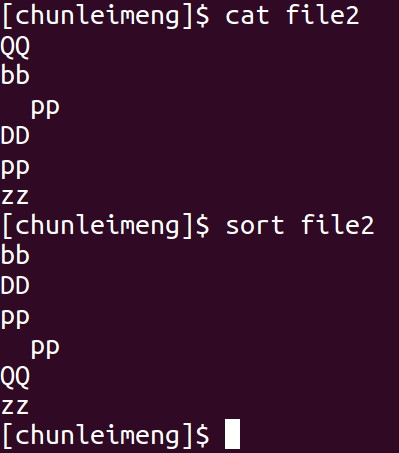
\includegraphics[scale=0.4]{pic1.png} \par

\section{按照数字排序(整数): sort -n}
~\\
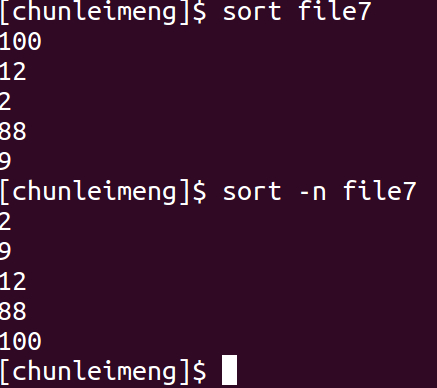
\includegraphics[scale=0.4]{pic2.png} \par

\section{逆序排序: sort -r}
~\\
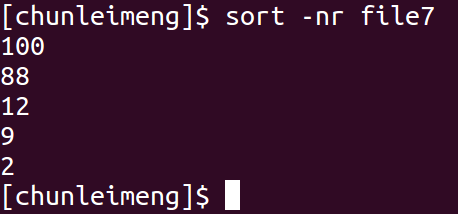
\includegraphics[scale=0.5]{pic3.png} \par

\section{按照月份排序: sort -M}
这个命令需要设置LC\_TIME为en\_EN.UTF-8
~\\
~\\
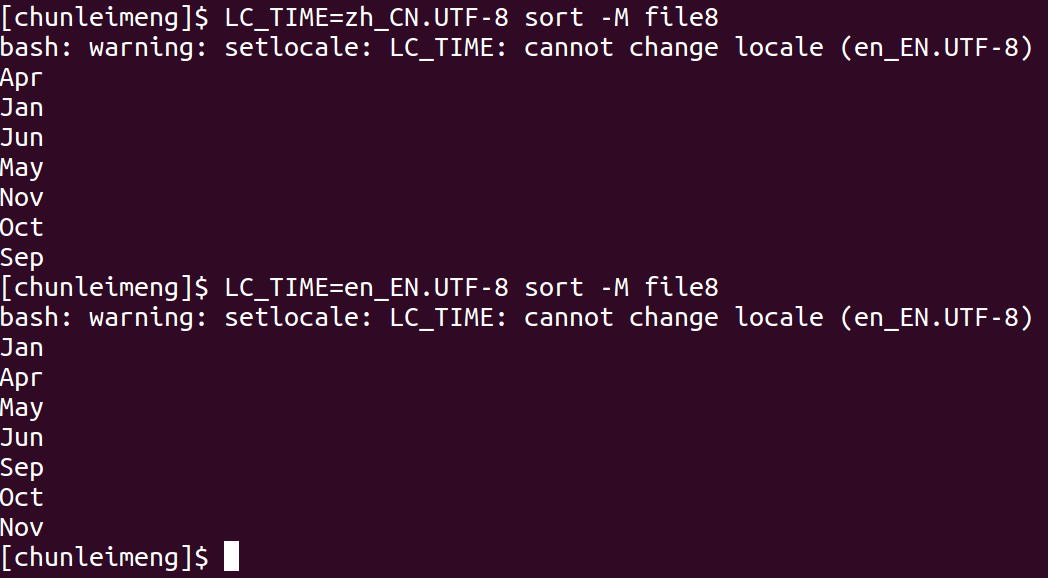
\includegraphics[scale=0.5]{pic4.png} \par

\section{合并两个已排序文件: sort -m, 去重: sort -u}
~\\
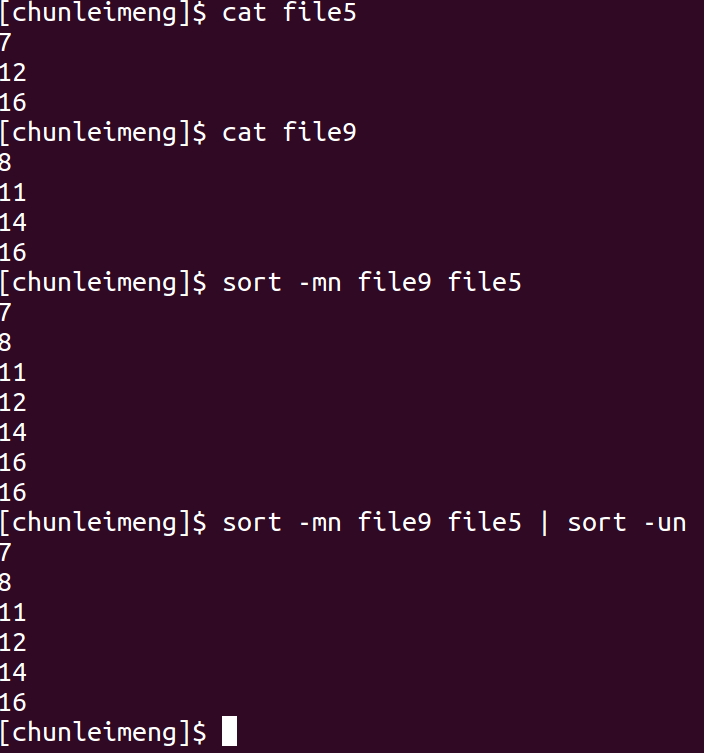
\includegraphics[scale=0.45]{pic5.png} \par

\section{随机化: sort -R}
~\\
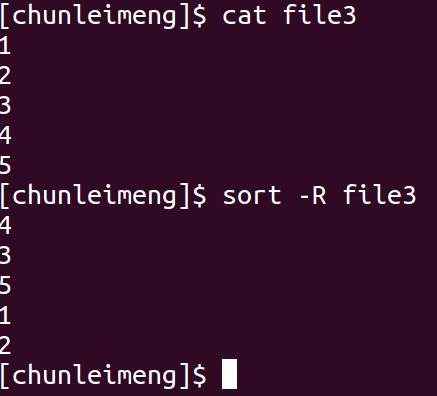
\includegraphics[scale=0.5]{pic6.png} \par

\section{指定排序字段: sort -k START[,END]}
把第二个字段当作数字排序\par
~\\
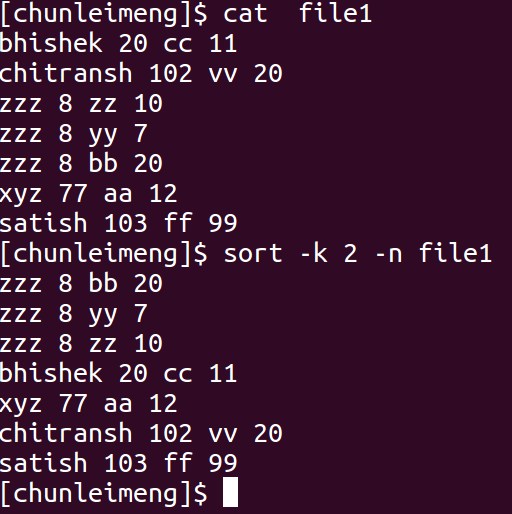
\includegraphics[scale=0.4]{pic7.png} \par
\section{指定分隔符: sort -t}
~\\
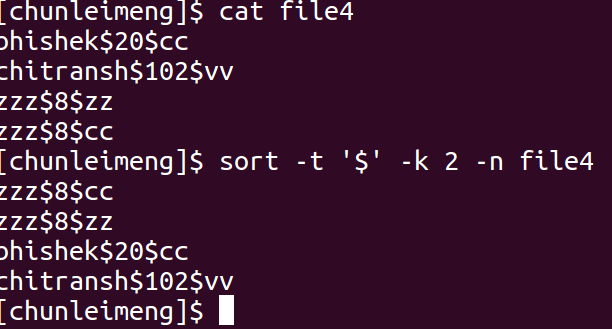
\includegraphics[scale=0.5]{pic8.png} \par

\section{按照多个列排序}
以第2列为第一关键字,以第4列为第二关键字排序 \par
~\\
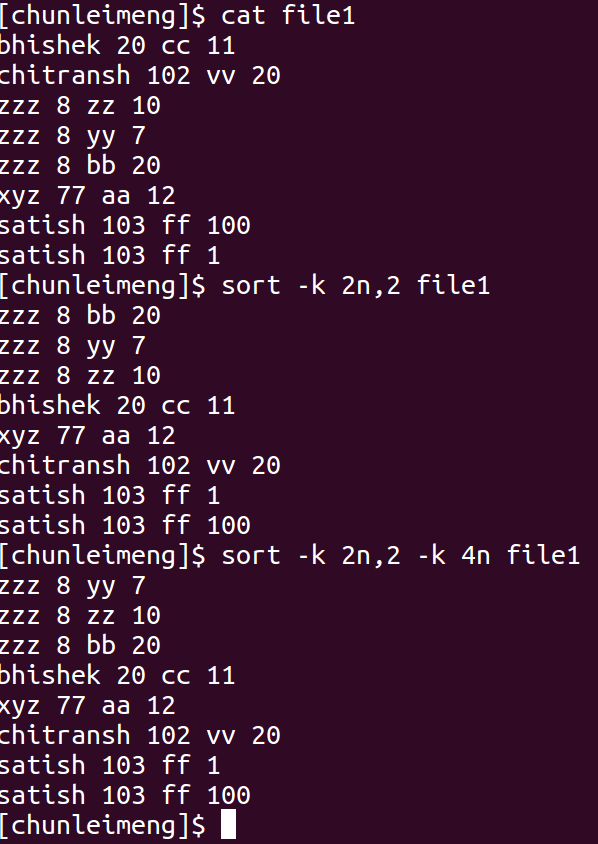
\includegraphics[scale=0.5]{pic10.png} \par

\section{按照浮点数排序: sort -g}
~\\
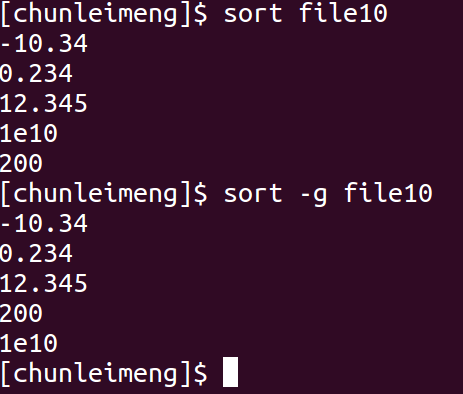
\includegraphics[scale=0.5]{pic9.png} \par
\end{document}
